\subsection{Physics}

\begin{wrapfigure}{!b}{4.0in}
  \vspace{-0.5cm} \centering \subfigure[Predictions of currents and
  temperature at 10m depth from a \texttt{HOPS} (Harvard Ocean
  Prediction System) model with assimilation of temperature and
  salinity measurements collected by CTD profiles and
  current-meters.]{\label{fig:model}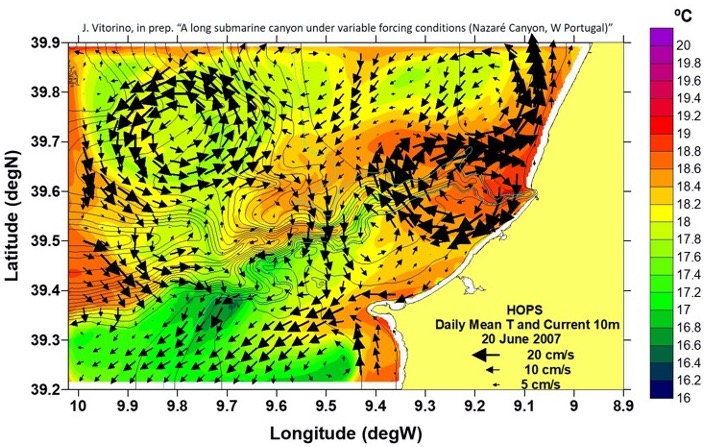
\includegraphics[scale=0.40]{fig/model.jpeg}}
  \subfigure[MUR SST image for June 20\textsuperscript{th} 2007. The
  red rectangle covers the area to be modeled in
  HOPS.]{\label{fig:SST}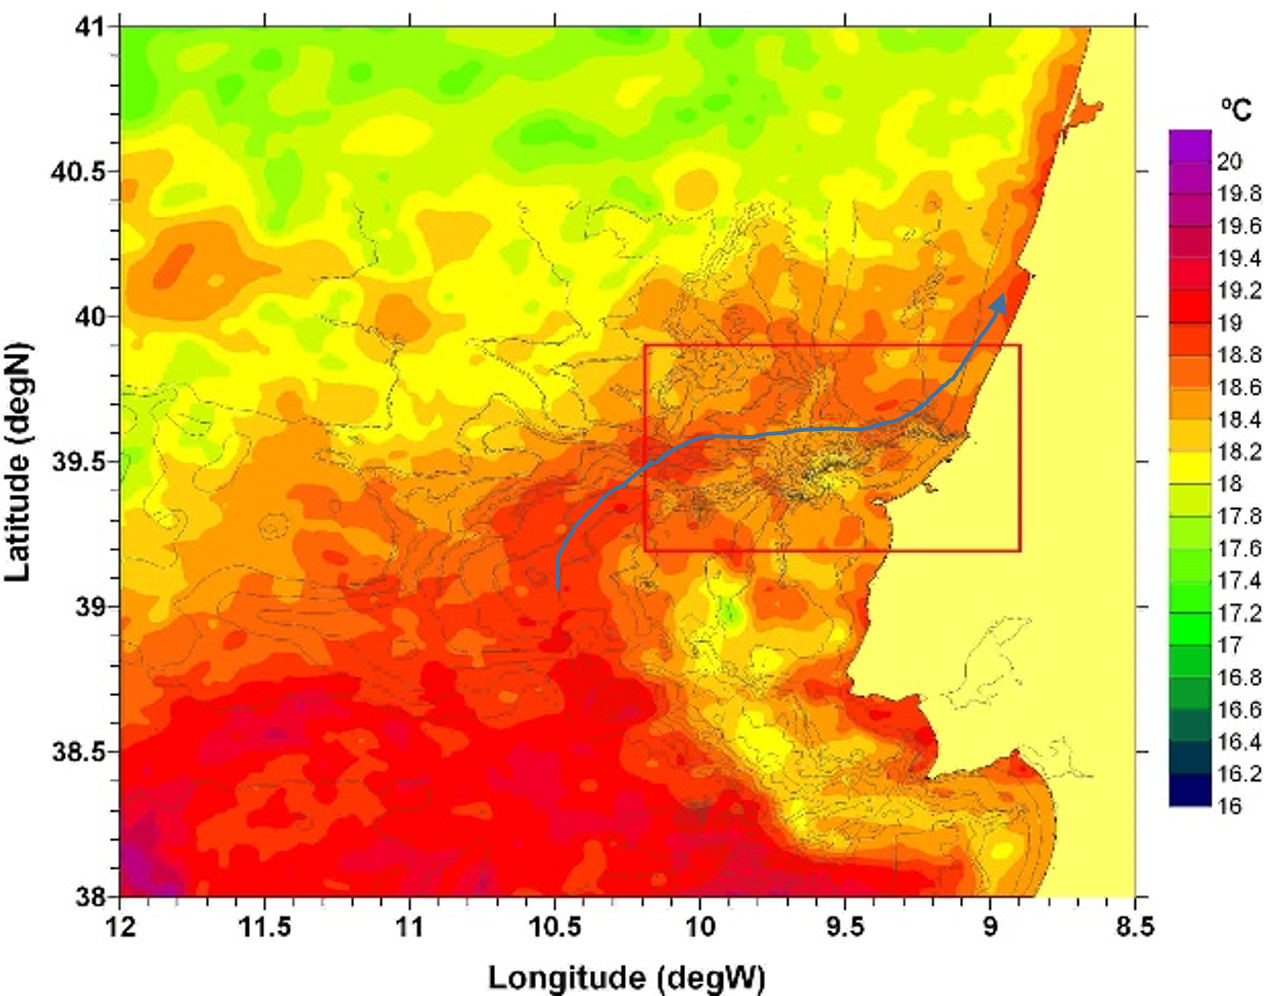
\includegraphics[scale=0.45]{fig/SST-Nazare.png}}
  \caption{}
\vspace{-0.5cm}
\end{wrapfigure}

The geographical domain in which \proj will focus on constitutes a key
area for the shaping of several main characteristics of the
shelf/slope oceanography of the northwestern Portuguese and Spanish
land-mass. The marked changes in the continental margin topography
that characterize this area play an important role in establishing the
nature of the shelf response to wind forcing or the adjustment of the
poleward slope intensified flow. The area (Fig. \ref{fig:model}) shows
several expressive examples of coastal mesoscale features such as the
large upwelling filament of Cabo Carvoeiro which is one of the larger
and more persistent features of the summer upwelling regime in the
western portuguese coast, with an expression similar to the large
filaments off of Cape Finisterre (northwestern Spanish coast), Cape da
Roca (near Lisbon) or Cape S.Vicente (in the southwestern tip of
Portugal).

The long and narrow \naz Canyon in addition promotes a rich variety of
coastal mesoscale and submesoscale processes that not only directly
affect the local ecosystems but can also contribute to impact a much
larger coastal ocean area. Since they are linked to the canyon
dynamics these processes develop on a relatively small area of the
coastal ocean which are associated with specific areas of the canyon
topography. In this way a strategy that concentrates several
observation systems in this small area can bring considerable insight
on the nature of the processes. This concentration is of particular
interest for \proj objectives. \kc{TO BE CONTINUED...\ldots}
 
 